\subsection{M.PC.1 - Percentuale di metriche soddisfatte}
\begin{figure}[H]
    \centering
    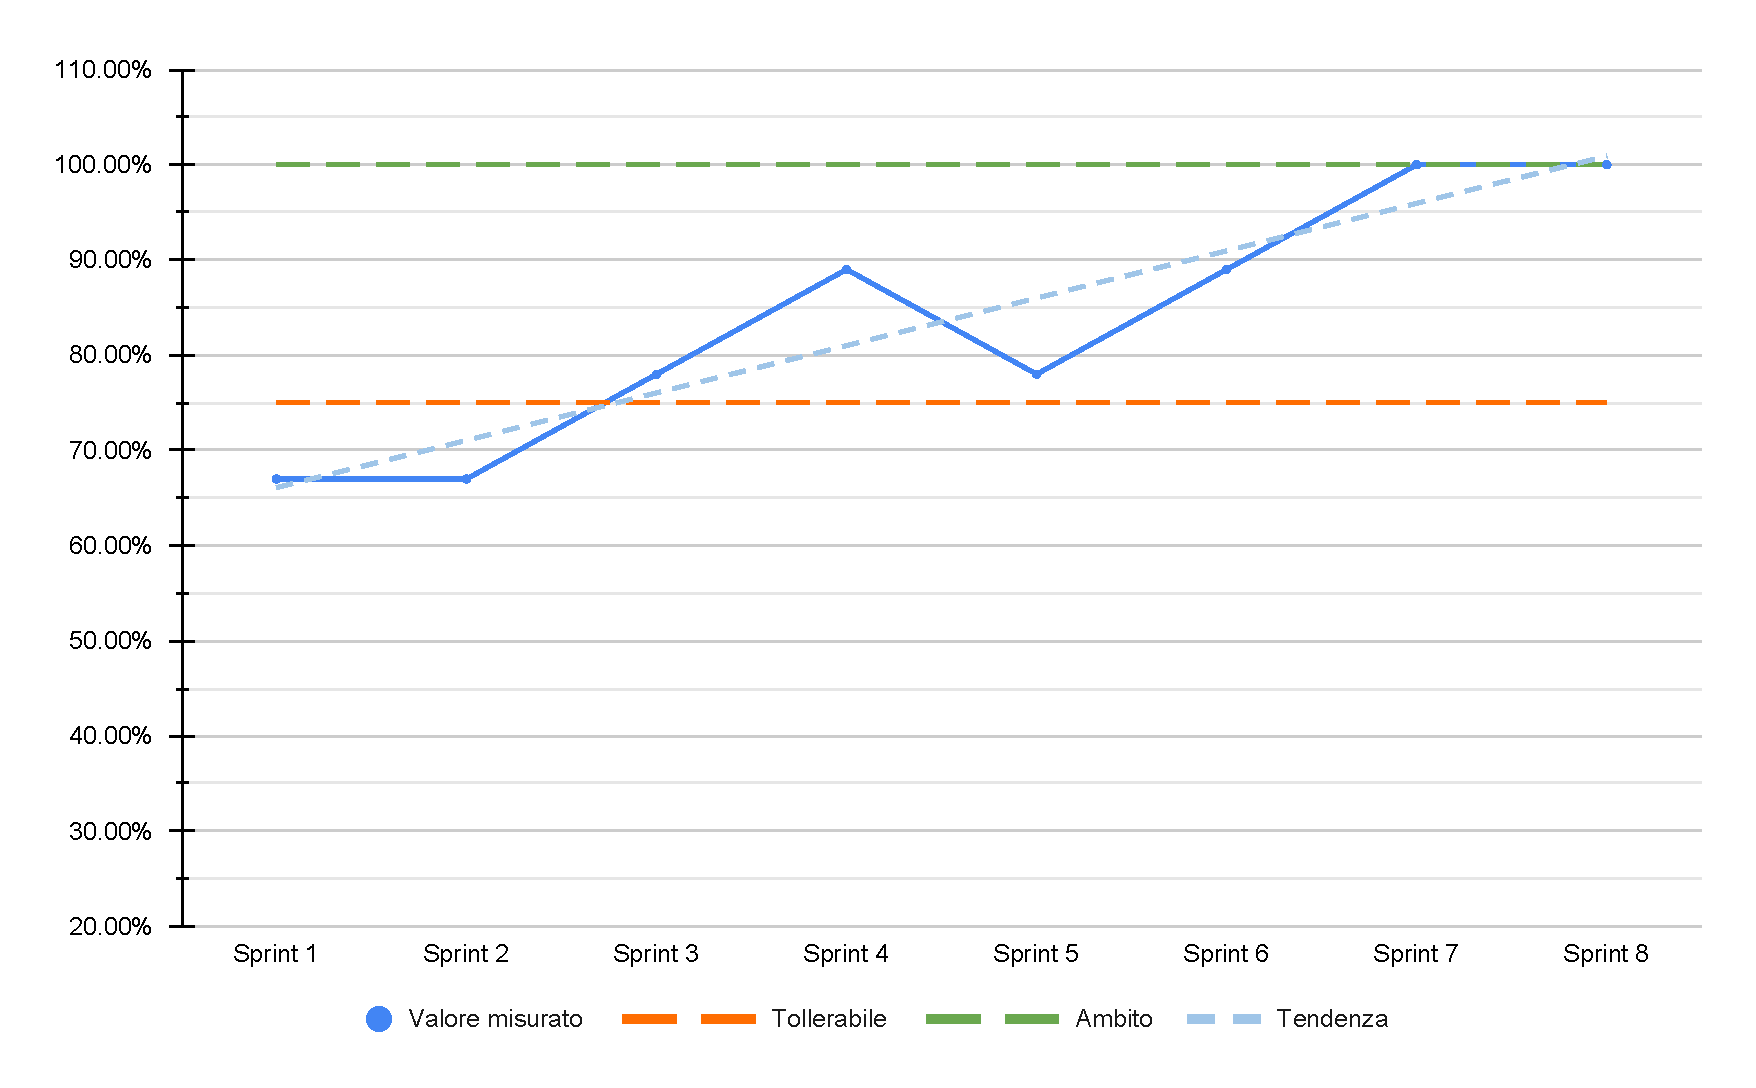
\includegraphics[width=\textwidth]{assets/metriche_soddisfatte.pdf}
    \caption{M.PC.1 - Percentuale di metriche soddisfatte}
\end{figure}

\par Il grafico evidenzia un inizio con risultati al di sotto delle previsioni, seguito da un miglioramento significativo nel corso degli \glossario{sprint}. All'inizio del periodo considerato, le metriche non raggiungevano gli obiettivi stabiliti, indicando possibili difficoltà iniziali nell'adattamento nei processi di lavoro, mentre il gruppo si abituava ai nuovi compiti o superava gli ostacoli iniziali. Tuttavia, nel corso degli \glossario{sprint} successivi, si nota un costante miglioramento delle metriche. Questo è dovuto all'implementazione di feedback migliorativi, all'adozione di pratiche più efficaci o all'accresciuta competenza e collaborazione all'interno del team.
Il grafico illustra un aumento graduale ma costante delle metriche nel tempo. Questo indica un miglioramento nella qualità del lavoro svolto e nel raggiungimento degli obiettivi di progetto, avvicinandosi alle aspettative iniziali del gruppo.
